\subsection{Архитектура на софтуерна програма}
Всяка софутерна програма изисква разработката на интерфейс, чрез който потребителя може да комуникира със програмата. Софтуерната програма е съставена от 4 модула, които комуникират помежду си, някои, от които имат визуална част, а други - не.
За разработката на софтуерната програма са използвани множество от практики за дизайн (design patterns), което позволява лесната поддръжка на софтуера за бъдеще \cite{patterns}.Имплементацията на модулите е реализирана чрез използването на широкоизползваната практика за дизайн - MVVM \cite{mvvm}. Предишната прекитка, предлага ясно разпределение между отговорностите на различните части на кода т.е код, които отговаря за логически операции не е свързан с код, който отговаря за обратната връзка между двете. Прадлага лесен начин за синхронизиране между логическата и визуалната част на дадена софтуерна програма чрез използване на "One way data binding" и "Two way data binding" похватите. 

\begin{figure}
    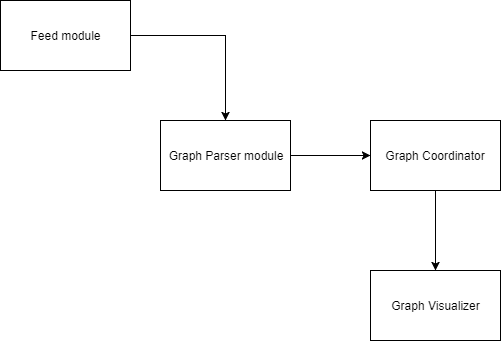
\includegraphics{modules}
    \caption{Архитектура на софтуерната програма}
    \label{fig:architecture}
\end{figure}

\begin{itemize}
    \item Options модул, който предлага начин за модифициране на различни настройки свързани с начина на изобразяване на обектите и тяхната начална конфигурация.
    \item Feed  модул, който има за отговорност да захранва с данни останалите модули с граф, който за всяка точка съдържа разстояниято между точката и всички останали точки. Ако разстоянието между две точки не може да бъде измерено то тогава разстоянието се означава с специален флаг поле, което е дефинирано като -безкрайност.
    \item Graph Parser модул, който има за цел да обработи информацията, която ‘Feed’ модулът изпраща и да я трансформира в друг граф – който държи информацията във върхове и дъги. Върховете и 
    дъгите съдържат информация, която помага за визуализацията на графа в 3D.
    \item Graph Coordinator модул, който има за цел да определи -координатите в пространството на всички обекти, които се съдържат в графа, който се получава в резултат на стъпка 2 (Graph Parser). Координатите се определят чрез система от линейни уравнения, които считат, че началната позиция на стационарните обекти е (0,0,0) - в един от ъглите на мястото, в което же бъдат следяни обектите.
    \item Graph Visualizer модул, който има за цел да използва графа, чиито координати са били вече определени от Graph Coordinator и да ги визуализира по удачен начин в 3 измерения.

\end{itemize}

\pagebreak

\subsection{Модул за опции}
Разработен е модул за опции, които позволява лесен контрол над началното разположение на статичните получатели в пространтвото. Модулът може да бъде използван чрез кликане на "Options" полето [фиг \ref{fig:options}]. Модулът изобразява презададен брой статични точки, чиито координати могат да бъдат зададени от потребителя на софтуерната програма. 

\begin{figure}
   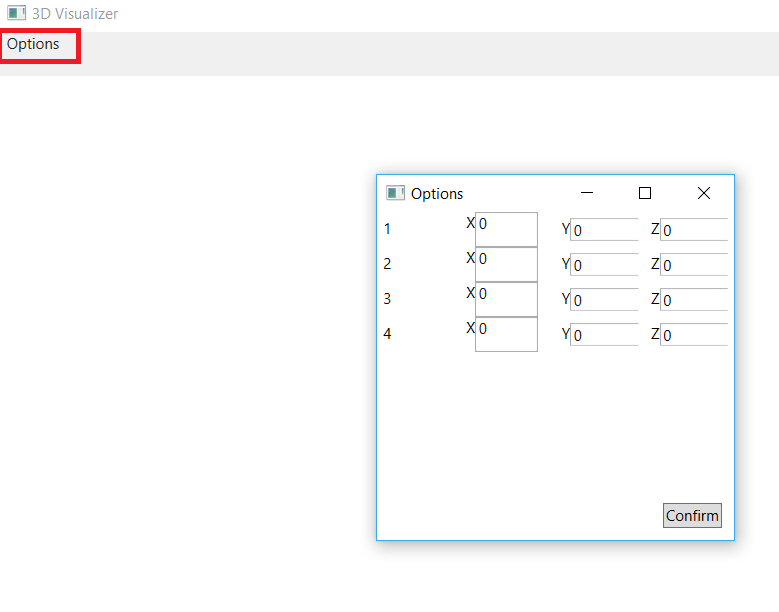
\includegraphics{OptionsLocation}
    \caption{Меню за опции}
    \label{fig:options}
\end{figure}

\pagebreak

\subsection{Feed модул}
Feed модулът има за цел да създаде граф, който съдържа дистанциите от всяка точка до всяка друга. Нуждата от възможност за лесна и бърза смяна между двата подхода наложи създаването на модула.\\\\
В процеса на работа бяха изградени 2 различни начина за получаване на данните от ултразвук трансмитери към ултразвук получатели. 
\begin{enumerate}
    \itemДанните се получават директно от физическите обекти. Стандартното измерване се случва чрез получаване на данните през сериен порт. Данните се предоставят от ултразвукови трансмитери и получатели в специален формат, който бива преобразуван към граф, съдържащ разстоянията между различните точки.
    \itemДанните биват генерирани чрез компютърен модел. Компютърния модел се състои от генератор на дистанции, който симулира движението на реален обект. Това се постига чрез манипулация на дистанцията между двойка (движещ,недвижещ) обект в пространството с константна стойност на определен интервал. Добавен е елемент на случайност, който позволява да се придаде по-реалистичен вид на движението на обектите.
\end{enumerate}

\pagebreak

\subsection{Graph Parser модул}
Graph Parser модулът има за цел да използва графа генериран от Feed модулът, за да създаде граф на свързаност, който съдържа
\begin{enumerate}
\itemВърхове, които представляват движещи/недвижещи се обекти 
\itemДъги, свързващи върховете, които означават съществуването на свързаност между
даден връх и друг връх.
\end{enumerate}

\pagebreak

\subsection{Graph Coordinator модул}
Целта на Graph Coordinator модула е да определи координатите в 3D на построения граф. Тази операция се извършва чрез минимизиране на бройката на възможните позиции използвайки система от уравнения. Всички възможни позиции се намират на радиус с дължина R (равен на дистанцията получена от сензора) на сфера. Задачата се трансформира:\\

\textit{За всеки получател се образуват K сфери (K=броя на трансмитерите), като сфера $x_i$ се центрира в позицията на на трансмитер с индекс $i$, а радиусът и е равен на измерената стойност за разстоянието между двата обекта. За да получим еднозначно решение ние трябва да елиминираме всички възможни позиции освен една. Всички решения на задачата за даден получател се намират на пресечния регион на всички сфери за дадения получател. Търси се такава конфигурация на позициите на всички получатели така че назначените позиции да не са в конфликт и броят на възможни решения за всяка позиция да е минимален.}\\\\

В 2D намирането на решения е лесно, поради следните причини:

\begin{enumerate}
    \itemБроят на пресечните точки на сферите при оптимално* позициониране на сензорите лесно може да бъде сведено до еднозначно решение.

    \itemВ 2-D пресечните точки на окръжностите са точки. В 3D пресечните точки се описват от 3D фигура. Това лесно може да бъде видяно на фигура \ref{spheres}.
\end{enumerate}

\begin{figure}
    \centerline{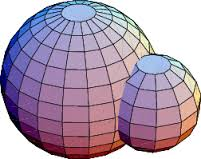
\includegraphics{spheres}}
    \caption{Пресечната точка на сфери в 3D е 3D регион от точки}
    \label{spheres}
\end{figure}

\pagebreak

\subsection{Graph Visualizer модул}
Целта на Graph Visualizer модула е да използва графа, чиито координати са били вече определени от Graph Coordinator и да ги визуализира по удачен начин в 3 измерения.


\subsection{Обобщение}
